\section{phase$\_$4}
	第四关的汇编代码如下:
	\begin{figure}[h]
		\centering
			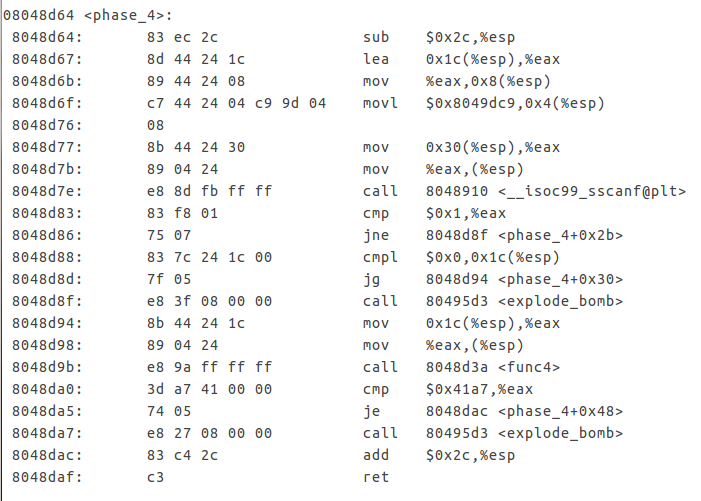
\includegraphics[scale=0.77]{images/phase_4.png}
	\end{figure}
	
	首先,它和phase$\_$3一样,调用了sscanf函数。和上一个函数的处理方法一样,运用gdb,发现sscanf的参数是\textbf{"$\%$d“},即读入一个整数n,存放在\textbf{0x1c($\%$esp)}。
	
	读入后,将n与0比较,如果$n \le 0$炸弹就会爆炸。
	
	因此,我们得到了第一个限制条件: $n > 0$
	
	随后,将n作为参数传入函数\textbf{func4}中。
	
	%一段代码
	
	这段代码表示,如果函数的返回值不为\textbf{0x41a7},则炸弹爆炸。
	
	这样就知道了第四关的要求:找出使\textbf{func4}的结果为\textbf{0x41a7}的输入值。
	
	于是我们开始研究\textbf{func4}函数。
	
	\begin{figure}[h]
		\centering
			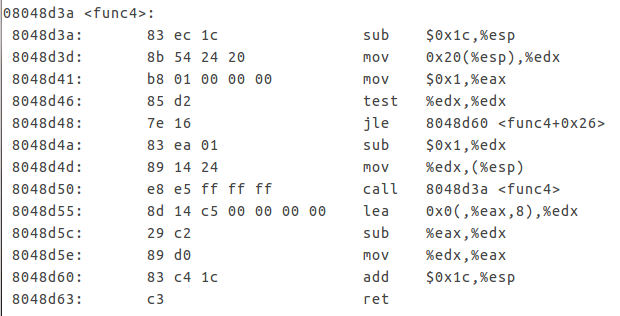
\includegraphics[scale=0.77]{images/fun_4.png}
	\end{figure}
	
	分析这一个函数,可以得出它的作用如下:
	
	\begin{itemize}
		\item	首先,函数将返回值置为1。
		\item	如果传入参数$x \le 0$,则直接返回。
		\item	递归调用\textbf{fun4}
		\item	将递归的结果乘7后作为返回值
	\end{itemize}
	
	对应的C语言代码如下:
	\lstinputlisting{sources/fun4.txt}
	
	因此,我们的问题变成:$\log_7(0x41a7)$ = ?
	
	经过计算得出,$7 ^ 5 = 16807 = 0x41a7$
	
	输入5,成功过关。